\section*{Encaminamiento por vector-distancia, direccionamiento IP y detecci\'on de errores con CRC}

\begin{enumerate}
    \item Aplique el algoritmo de encaminamiento de vector-distancia a la siguiente topolog\'ia de red.
    \begin{enumerate}
        \item Indique el estado de las tablas de ruteo para las etapas de cold-start y luego para el env\'io de los primeros
        dos mensajes.
        \item[] \textbf{Tablas de rutio para la etapa cold-start}
        \begin{table}[H]
            \begin{tabular}{@{}clcll@{}}
                \toprule
                From A to            & \multicolumn{1}{c}{Link} & Cost                 \\ \midrule
                A                    & local                    & 0                    \\ \bottomrule
            \end{tabular}
            \hfill
            \begin{tabular}{@{}clcll@{}}
                \toprule
                From B to            & \multicolumn{1}{c}{Link} & Cost                 \\ \midrule
                B                    & local                    & 0                    \\ \bottomrule
            \end{tabular}
            \hfill
            \begin{tabular}{@{}clcll@{}}
                \toprule
                From C to            & \multicolumn{1}{c}{Link} & Cost                 \\ \midrule
                C                    & local                    & 0                    \\ \bottomrule
            \end{tabular}
        \end{table}
        \begin{table}[H]
            \begin{tabular}{@{}clcll@{}}
                \toprule
                From D to            & \multicolumn{1}{c}{Link} & Cost                 \\ \midrule
                D                    & local                    & 0                    \\ \bottomrule
            \end{tabular}
            \hfill
            \begin{tabular}{@{}clcll@{}}
                \toprule
                From E to            & \multicolumn{1}{c}{Link} & Cost                 \\ \midrule
                E                    & local                    & 0                    \\ \bottomrule
            \end{tabular}
            \hfill
            \begin{tabular}{@{}clcll@{}}
                \toprule
                From F to            & \multicolumn{1}{c}{Link} & Cost                 \\ \midrule
                F                    & local                    & 0                    \\ \bottomrule
            \end{tabular}
        \end{table}

        \item[] \textbf{Tablas de ruteo suponiendo que A inicia con el env\'io de mensajes}
        \begin{table}[H]
            \begin{tabular}{@{}clcll@{}}
                \toprule
                From A to            & \multicolumn{1}{c}{Link} & Cost                 \\ \midrule
                A                    & local                    & 0                    \\ \bottomrule
            \end{tabular}
            \hfill
            \begin{tabular}{@{}clcll@{}}
                \toprule
                From B to            & \multicolumn{1}{c}{Link} & Cost                 \\ \midrule
                B                    & local                    & 0                    \\ 
                A                    & 1                        & 1                    \\ \bottomrule
            \end{tabular}
            \hfill
            \begin{tabular}{@{}clcll@{}}
                \toprule
                From C to            & \multicolumn{1}{c}{Link} & Cost                 \\ \midrule
                C                    & local                    & 0                    \\ 
                A                    & 3                        & 1                    \\ \bottomrule
            \end{tabular}
        \end{table}
        \begin{table}[H]
            \begin{tabular}{@{}clcll@{}}
                \toprule
                From D to            & \multicolumn{1}{c}{Link} & Cost                 \\ \midrule
                D                    & local                    & 0                    \\ 
                A                    & 4                        & 1                    \\ \bottomrule
            \end{tabular}
            \hfill
            \begin{tabular}{@{}clcll@{}}
                \toprule
                From E to            & \multicolumn{1}{c}{Link} & Cost                 \\ \midrule
                E                    & local                    & 0                    \\ \bottomrule
            \end{tabular}
            \hfill
            \begin{tabular}{@{}clcll@{}}
                \toprule
                From F to            & \multicolumn{1}{c}{Link} & Cost                 \\ \midrule
                F                    & local                    & 0                    \\ \bottomrule
            \end{tabular}
        \end{table}

        \item[] \textbf{Tablas de ruteo suponiendo que B es el segundo nodo en enviar mensaje}
        \begin{table}[H]
            \begin{tabular}{@{}clcll@{}}
                \toprule
                From A to            & \multicolumn{1}{c}{Link} & Cost                 \\ \midrule
                A                    & local                    & 0                    \\
                B                    & 1                        & 1                    \\ \bottomrule
            \end{tabular}
            \hfill
            \begin{tabular}{@{}clcll@{}}
                \toprule
                From B to            & \multicolumn{1}{c}{Link} & Cost                 \\ \midrule
                B                    & local                    & 0                    \\ 
                A                    & 1                        & 1                    \\ \bottomrule
            \end{tabular}
            \hfill
            \begin{tabular}{@{}clcll@{}}
                \toprule
                From C to            & \multicolumn{1}{c}{Link} & Cost                 \\ \midrule
                C                    & local                    & 0                    \\ 
                A                    & 3                        & 1                    \\
                B                    & 2                        & 1                    \\ \bottomrule
            \end{tabular}
        \end{table}
        \begin{table}[H]
            \begin{tabular}{@{}clcll@{}}
                \toprule
                From D to            & \multicolumn{1}{c}{Link} & Cost                 \\ \midrule
                D                    & local                    & 0                    \\ 
                A                    & 4                        & 1                    \\ \bottomrule
            \end{tabular}
            \hfill
            \begin{tabular}{@{}clcll@{}}
                \toprule
                From E to            & \multicolumn{1}{c}{Link} & Cost                 \\ \midrule
                E                    & local                    & 0                    \\ \bottomrule
            \end{tabular}
            \hfill
            \begin{tabular}{@{}clcll@{}}
                \toprule
                From F to            & \multicolumn{1}{c}{Link} & Cost                 \\ \midrule
                F                    & local                    & 0                    \\ \bottomrule
            \end{tabular}
        \end{table}

        \item Luego, indique el estado de las tablas de ruteo para el estado estacionario.
        \item[] \textbf{Para llegar a esta tabla se considero el orden alafab\'etico para el env\'io de mensajes}
        \begin{table}[H]
            \begin{tabular}{@{}clcll@{}}
                \toprule
                From A to            & \multicolumn{1}{c}{Link} & Cost                 \\ \midrule
                A                    & local                    & 0                    \\
                B                    & 1                        & 1                    \\ 
                C                    & 3                        & 1                    \\
                D                    & 4                        & 1                    \\ 
                E                    & 3                        & 2                    \\ 
                F                    & 3                        & 2                    \\ \bottomrule
            \end{tabular}
            \hfill
            \begin{tabular}{@{}clcll@{}}
                \toprule
                From B to            & \multicolumn{1}{c}{Link} & Cost                 \\ \midrule
                B                    & local                    & 0                    \\ 
                A                    & 1                        & 1                    \\ 
                C                    & 2                        & 1                    \\
                D                    & 1                        & 2                    \\
                E                    & 2                        & 2                    \\
                F                    & 2                        & 2                    \\ \bottomrule
            \end{tabular}
            \hfill
            \begin{tabular}{@{}clcll@{}}
                \toprule
                From C to            & \multicolumn{1}{c}{Link} & Cost                 \\ \midrule
                C                    & local                    & 0                    \\ 
                A                    & 3                        & 1                    \\
                B                    & 2                        & 1                    \\ 
                D                    & 5                        & 2                    \\ 
                E                    & 5                        & 1                    \\ 
                F                    & 6                        & 1                    \\ \bottomrule
            \end{tabular}
        \end{table}
        \begin{table}[H]
            \begin{tabular}{@{}clcll@{}}
                \toprule
                From D to            & \multicolumn{1}{c}{Link} & Cost                 \\ \midrule
                D                    & local                    & 0                    \\ 
                A                    & 4                        & 1                    \\ 
                B                    & 4                        & 2                    \\
                C                    & 7                        & 2                    \\
                E                    & 7                        & 1                    \\ 
                F                    & 7                        & 2                    \\ \bottomrule
            \end{tabular}
            \hfill
            \begin{tabular}{@{}clcll@{}}
                \toprule
                From E to            & \multicolumn{1}{c}{Link} & Cost                 \\ \midrule
                E                    & local                    & 0                    \\
                A                    & 5                        & 2                    \\
                B                    & 5                        & 2                    \\
                C                    & 5                        & 1                    \\ 
                D                    & 7                        & 1                    \\ 
                F                    & 8                        & 1                    \\ \bottomrule
            \end{tabular}
            \hfill
            \begin{tabular}{@{}clcll@{}}
                \toprule
                From F to            & \multicolumn{1}{c}{Link} & Cost                 \\ \midrule
                F                    & local                    & 0                    \\ 
                A                    & 6                        & 2                    \\
                B                    & 6                        & 2                    \\ 
                C                    & 6                        & 1                    \\
                D                    & 8                        & 2                    \\
                E                    & 8                        & 1                    \\ \bottomrule
            \end{tabular}
        \end{table}

        \item Una vez alcanzado el estado estacionario , el enlace 6 se rompe. Describa la manera en c\'omo procede el protocolo
        hasta retomar un nuevo estado estacionario.
        \item ¿Qu\'e fen\'omeno podr\'ia causar un bucle de ruteo?
        \item Finalmente, ¿cu\'al protocolo en la pr\'actica implementa el algoritmo de vector-distancia? ¿cu\'al es la frecuencia
        de los mensajes de refresco y cu\'al es la finalidad de los mismos?

        \begin{figure}[H]
            \centering
            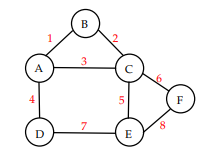
\includegraphics[width=0.35\textwidth]{img/Vector-distancia.png}
        \end{figure}
    \end{enumerate}

    \item Suponga que le han asignado el bloque de red 132.46.0.0/16 y que necesita configurar ocho subredes.
    \begin{enumerate}
        \item ¿Cu\'antos d\'igitos binarios se requieren para definir ocho subredes?
        \item Especifique el prefijo de red extendido que permite la creaci\'on de las 8 subredes.
        \item Exprese las direcciones de subred en formato binario y decimal.
        \item Enliste el rango de direcciones IP que pueden asignarse a la subred n\'umero 4.
        \item ¿Cu\'al es la direcci\'on de difusi\'on (\textit{broadcast}) de la subred n\'umero 4?
    \end{enumerate}

    \item Suponga que se le ha asignado el bloque de direcciones de red 200.30.1.0/24.
    \begin{enumerate}
        \item Defina un prefijo de red extendido que permita crear 20 estaciones en cada subred.
        \item ¿Cu\'al es el n\'umero m\'aximo de estaciones que pueden asignarse a cada subred?
        \item ¿Cu\'al es el n\'umero m\'aximo de subredes que pueden definirse?
        \item Especifique las subredes de 200.30.1.0/24 en formatos binario y decimal.
        \item Enliste las direcciones de estaci\'on que pueden asignarse a la subred 6.
        \item ¿Cu\'al es la direcci\'on de difusi\'on para la subred 2?
    \end{enumerate}

    \item Se le ha asignado a una organizaci\'on el n\'umero de red 140.20.0.0/16 y \'esta planea desarrollar VLSM. En el primer
    nivel de jerarqu\'ia, se necesitan configurar ocho subredes. La subred 1 necesita configurar 32 sub-redes y la subred 6
    necesita configurar 16 sub-redes. Finalmente, la sub-red 6-14 necesita configurar 8 \(sub^2-subredes\).
    \begin{enumerate}
        \item Dibuje el \'arbil que ilustre la jerarqu\'ia necesaria para implementar VLSM.
        \item Especifique las ocho subredes 140.20.0.0/16.
        \item Enliste las direcciones de estaci\'on que pueden asignarse a la subred 3.
        \item Indique la direcci\'on de difusi\'on de la subred 3.
        \item Indique las 16 sub-redes de la subred 6.
        \item Enliste las direcciones de estaci\'on que pueden asignarse a la sub-subred 6-3.
        \item Indentifique la direcci\'on de broadcast para la sub-subred 6-3.
        \item Especifique las ocho \(sub^2-subredes\) de la sub-subred 6-14.
        \item Enliste las direcciones de estaci\'on que pueden asignarse en la \(sub^2-subred\) 6-14-2.
        \item Indentifique la direcci\'on de broadcast de la \(sub^2-subred\) 6-14-2.
    \end{enumerate}

    \item En el nivel de enlace de datos se utiliza frecuentemente el mecanismo de verificaci\'on de redundancia c\'iclica 
    (\textit{CRC: Cyclic Redundance Check}) para que una interfaz receptora concluya sobre si la trama recibida, \(T'\) contiene
    o no errores. Suponga que el mensaje a transmitir es \(M=1101011011\) y que el generador es \(G=10011\).
    \begin{enumerate}
        \item Encuentre la trama, \(T\) que env\'ia el transmisor.
        \item Realice la operaci\'on que ejecuta la interfaz receptora si el patr\'on de error inducido en el canal
        \(e=00000000000000\), ¿cu\'al es la conclusi\'on del receptor?
        \item Realice lo mismo que en (b), pero ahora con un error inducido en el canal f\'isico \(e=00100000010011\), 
        ¿cu\'al es la conclusi\'on del receptor?
        \item ¿Existe la posibilidad de que habiendo errores en \(T'\), la trama recibida, el receptor sea incapaz de detectarlos?
        Explique.
        \item Finalmente, realice (a)-(c) operando polinimialmente.
    \end{enumerate}
\end{enumerate}